%        File: hello.tex
%     Created: Tue Nov 08 02:00 PM 2022 W
% Last Change: Tue Nov 08 02:00 PM 2022 W
%
\documentclass[portuguese,11pt,a4paper,titlepage]{article}

%\usepackage{titling}
\usepackage{graphicx}
\usepackage{fancyhdr}
\usepackage[portuguese]{babel}
\usepackage{blindtext}
\usepackage{color}
\usepackage{listings}
\usepackage[T1]{fontenc}
\usepackage[margin=3cm]{geometry}
\usepackage[final]{pdfpages}
\usepackage{siunitx}
\usepackage[framed, numbered]{matlab-prettifier}
\usepackage{wrapfig}
\usepackage{subcaption}

\newcommand{\nextyear}{\advance\year by 1 \the\year\advance\year by -1}

\setlength{\headheight}{14.2pt}
\fancypagestyle{fancy}{
	\fancyhf{}
	\fancyhead[C]{A01 - speed\_run}
	\fancyfoot[R]{
		\textsf{\thepage}
	}
	\fancyfoot[L]{
		\textsf{AED - \the\year/\nextyear}
	}
	\fancyfoot[C]{
\includegraphics[height=.8cm]{ua.pdf}}
	\renewcommand{\headrulewidth}{0pt}
}
\pagestyle{fancy}

\definecolor{mygreen}{rgb}{0,0.6,0}
\definecolor{mygray}{rgb}{0.5,0.5,0.5}
\definecolor{mymauve}{rgb}{0.58,0,0.82}

\lstdefinestyle{c_without_comments}%
{
	  style=c_with_comments,
	    morecomment  = [l][\@gobble]{//},
		  morecomment  = [is]{/*}{*/},
}
\lstset{ 
	backgroundcolor=\color{white},   % choose the background color; you must add \usepackage{color} or \usepackage{xcolor}; should come as last argument
	basicstyle=\small\ttfamily,        % the size of the fonts that are used for the code
	breakatwhitespace=false,         % sets if automatic breaks should only happen at whitespace
	breaklines=true,                 % sets automatic line breaking
	captionpos=b,                    % sets the caption-position to bottom
	commentstyle=\color{mygreen},    % comment style
	extendedchars=true,              % lets you use non-ASCII characters; for 8-bits encodings only, does not work with UTF-8
	frameround=tttt,
	frame=single,	                   % adds a frame around the code
	keepspaces=true,                 % keeps spaces in text, useful for keeping indentation of code (possibly needs columns=flexible)
	keywordstyle=\color{blue},       % keyword style
	language=C,                 % the language of the code
	morekeywords={*,\ldots},            % if you want to add more keywords to the set
	numbers=left,                    % where to put the line-numbers; possible values are (none, left, right)
	numbers=none,
	rulecolor=\color{black},         % if not set, the frame-color may be changed on line-breaks within not-black text (e.g. comments (green here))
	showspaces=false,                % show spaces everywhere adding particular underscores; it overrides 'showstringspaces'
	showstringspaces=false,          % underline spaces within strings only
	showtabs=false,                  % show tabs within strings adding particular underscores
	stringstyle=\color{mymauve},     % string literal style
	tabsize=2,	                   % sets default tabsize to 2 spaces
}


\newcommand{\extrang}[1]{\textit{#1}}
\newcommand{\srcdir}{..}
\newcommand{\matlabdir}{"../MATLAB-fittings"}

\title{ \normalsize Licenciatura em Engenharia Informática\vskip 1.5em
		\Huge Algoritmos e Estruturas de Dados\vskip .7em
		\bfseries speed\_run\vskip 1.5em
		
\includegraphics{ua.pdf}
}
\author{
	João Catarino\\NMec: 93096\and Rúben Garrido\\NMec: 107927\and Nuno Vieira\\NMec: 107283
}
\date{\today}

\begin{document}
%\begin{titlingpage}
\maketitle
%\end{titlingpage}
\section{Introdução}
Este trabalho tem como objetivo desenvolver algoritmos que sejam capazes
de encontrar o menor número de passos necessários para resolver o seguinte problema:
\section{Soluções}
A solução original utiliza uma função recursiva para verificar todas as combinações
de passos a todas as velocidades possíveis dentro dos limites de cada casa,
guardando sempre a melhor solução encontrada até ao momento. Esta possui um tempo
de execução com ordem de grandeza \begin{math}10^{154}\end{math} (em anos) para a resolução do caso \begin{math}n = 800\end{math}.
Com vista em obter a solução em tempo aceitável, criámos duas soluções capazes de
o fazer na ordem dos microsegundos. A primeira altera apenas ligeiramente a
solução original. A segunda é não recursiva e utiliza o princípio da solução anterior com
algumas optimizações.
\subsection{Original}
A solução dada é uma solução recursiva que itera sobre todas as possibilidades de
percurso, guardando a melhor solução até ao momento.

Esta parte das soluções de maior número de passos (menor velocidade por passo) para
as de menor número de passos (maior velocidade por passo) dentro das regras do problema.

Pelo facto de a solução ser recursiva, à medida que o tamanho do problema aumenta,
o número de chamadas recursivas também aumenta, o que leva a um tempo de execução exponencial.
Por exemplo, a partir de \begin{math}n = 35\end{math}, o tempo de execução é superior a 1 segundo,
pelo que esta não é, portanto, uma solução viável para o problema. 

\subsection{Original Improved}
Esta solução introduz duas pequenas mudanças no código original, que, no entanto,
geram alterações significativas no seu comportamento.

Em primeiro lugar, é introduzido controlo de fluxo através de um valor de retorno
\extrang{boolean} (implementado como inteiro).
\lstinputlisting[linerange={167-169}]{\srcdir/speed\_run.c}
Se uma sequência de chamadas recursivas chegar a uma solução, a última chamada
retorna 1. \lstinputlisting[linerange={166-167}]{\srcdir/speed\_run.c}
Se for este o caso, as chamadas anteriores retornarão também 1.
Isto significa que o programa grava apenas a primeira solução que encontrar.
\lstinputlisting[linerange={153-158}]{\srcdir/speed\_run.c}
Tendo isto, torna-se imperativo que o programa encontre a melhor solução possível
à primeira tentativa. Isto implica que o ``carro'' se mova o mais rápido possível
em qualquer passo para obter o menor número de passos. A segunda alteração
garante essa condição ao fazer com que o programa itere
desde as maiores velocidades para as menores.
\lstinputlisting[linerange={163-164}]{\srcdir/speed\_run.c}

\subsection{Advance and retreat}
Este algoritmo foi feito de raiz. Tem como
princípio tentar a qualquer passo avançar com a velocidade mais alta.
Em cada passo, a escolha de velocidade é representada por um incremento
($-$1, 0 ou 1). O programa começa sempre por tentar o maior incremento.
Para verificar passos possíveis, utilizam-se os seguintes métodos:

Calcular a distância de paragem para cada velocidade possível em cada passo para evitar correr para além do fim do
trajeto:
\lstinputlisting[firstline=125, lastline=135]{\srcdir/speed\_run.c}

Verificar, a partir do incremento mais alto, se uma ``passada'' não  quebra
os limites de velocidade das casas pelas quais passaria:
\lstinputlisting[firstline=196, lastline=203]{\srcdir/speed\_run.c}

Feito o passo, a escolha de incremento é guardada num \extrang{array}
na posição associada ao número do passo. Desta forma, este \extrang{array}
guarda as escolhas feitas até ao passo atual.
Quando um passo é impossível de executar a qualquer das velocidades possíveis nesse
passo, o algoritmo recua um passo e tenta reduzir o incremento de velocidade até que
consiga avançar novamente. Não sendo possível avançar com nenhum dos incrementos,
o programa recua novamente, e assim sucessivamente.
\pagebreak
\subsection{Combined}
Some text here
\pagebreak

\section{PDFs de soluções}
\subsection{Original Improved}
\includegraphics[width=\textwidth]{800_2.pdf}
\subsection{Advance and retreat}
\includegraphics[width=\textwidth]{800_3.pdf}
\subsection{Combined}
\includegraphics[width=\textwidth]{800_4.pdf}
\pagebreak

\section{Tempos de execução e estimativas}
\subsection{Original}
Devido à complexidade do algoritmo, não foi possível obter tempos de execução para \begin{math}n = 800\end{math},
pelo que foi necessário recorrer a estimativas, utilizando o MATLAB.

Em primeiro lugar, procedeu-se ao ajuste de uma função exponencial aos tempos obtidos
até \begin{math}n = 50\end{math}.
Dado o enorme salto existente de \begin{math}n = 50\end{math} para \begin{math}n = 55\end{math},
a função a ajustar teria de ser do tipo \begin{math}a\times e^{bx}\end{math}.
Assim, utilizando a Curve Fitting Toolbox do MATLAB, obteve-se,
para o percurso gerado com o número mecanográfico 107927,
a seguinte equação: \begin{math}y = (\num{6.231e-08})\times e^{0.4869x}\end{math}.

Possuindo uma função exponencial que se ajusta aos valores obtidos, foi possível,
portanto, estimar os tempos de execução para \begin{math}n = 800\end{math}.
Deste modo, o tempo de execução previsto é de \num{9.23397e+161} segundos,
o que equivale a, aproximadamente, \num{2.96874e+154} anos.

\begin{figure}[h]
	\begin{subfigure}{0.47\textwidth}
	\includegraphics[width=\linewidth]{\matlabdir/Results\_original/107927\_Original\-and\-fitted.png} 
	\caption{Tempos de execução obtidos e função exponencial ajustada.}
	\label{fig:subim1}
	\end{subfigure}
	\hspace{0.049\textwidth}
	\begin{subfigure}{0.47\textwidth}
	\includegraphics[width=\linewidth]{\matlabdir/Results\_original/107927\_800.png}
	\caption{Tempo de execução estimado, recorrendo à função ajudada em (a), para \begin{math}n=800\end{math}.}
	\label{fig:original_800}
	\end{subfigure}
	
	\caption{Tempos de execução para o algoritmo original.}
	\vspace{-20pt}
	\label{fig:original}
\end{figure}

\subsection{Original Improved}
\begin{wrapfigure}[14]{r}{0.47\textwidth}
	\vspace{-13pt}
	\includegraphics[width=\linewidth]{\matlabdir/Results\_sol2/fitted.png}
	\caption{Tempos de execução e função exponencial ajustada.}
	\label{fig:sol2}
\end{wrapfigure}
	
Pelo facto de o algoritmo Original Improved efetuar cálculos em tempos com ordem de grandeza
\begin{math}10^{-6}\end{math}, foi possível obter um tempo de execução para \begin{math}n = 800\end{math}.

Contudo, os valores até \begin{math}n = 300\end{math} não são fiáveis para ajustar uma reta,
pois são constituídos, na sua grande parte, por ruído.
Este é causado pelo script de medição de tempo que, devido a questões de arquitetura,
não consegue reportar valores temporais tão baixos.

A reta de ajuste foi obtida através da Curve Fitting Toolbox do MATLAB, ao qual se determinou
a sua equação \begin{math}y=(\num{4.341e-09})x+(\num{1.151e-06})\end{math}.
\pagebreak
\subsection{Advance and retreat}
Tal como a solução anterior, o algoritmo Advance and retreat efetua cálculos em tempos bastante baixos
(ordem de grandeza \begin{math}10^{-6}\end{math}), até \begin{math}n = 800\end{math}.
Assim, os valores iniciais de \begin{math}n\end{math} constituem igualmente ruído.

A reta de ajuste foi obtida através da Curve Fitting Toolbox do MATLAB, ao qual se determinou
a sua equação \begin{math}y=(\num{8.001e-09})x+(\num{1.912e-06})\end{math}.
\begin{figure}[h]
	\centering
	\includegraphics[width=0.5\linewidth]{\matlabdir/Results\_sol3/fitted.png}
	\caption{Tempos de execução e função exponencial ajustada.}
	\label{fig:sol2}
\end{figure}

\subsection{Combined}
Some text here
\pagebreak

\section{Código}
\subsection{Original Improved}
\lstinputlisting[firstline=142, lastline=184]{\srcdir/speed\_run.c}
\pagebreak
\subsection{Advance and retreat}
\lstinputlisting[firstline=192, lastline=280]{\srcdir/speed\_run.c}
\pagebreak
\subsection{Combined}
\lstinputlisting[firstline=289, lastline=331]{\srcdir/speed\_run.c}
\pagebreak
\subsection{Ajuste dos dados obtidos utilizando o MATLAB}
\lstinputlisting[firstline=5, lastline=31, style=Matlab-editor, numbers=none, basicstyle=\small\ttfamily]{\matlabdir/speed\_run.m}

\end{document}
